\documentclass[11pt,twocolumn]{article}
\usepackage{geometry}
\usepackage{ctex}
\usepackage{graphicx}
\usepackage{algorithm}
\usepackage{algorithmic}
\usepackage{amssymb}
\usepackage{amsmath}
\usepackage{hyperref}
\geometry{left=2.5cm,right=2.5cm,top=2.5cm,bottom=2.5cm}

\begin{document}
\title{\textbf{轨迹预测暑期项目} \\ \small{\kaishu 阶段性报告:Markov轨迹预测实现}}
\author{刘前\hspace{2em}liuqian14@mails.tsinghua.edu.cn}
\maketitle

近两周尝试使用Markov链对用户的轨迹进行建模与预测。主要工作是:

1.分析数据,获取\textbf{轨迹数据的基本分布}(轨迹长度和时间分布);

2.实现基于Markov链的轨迹预测算法:

a)	使用\texbf{经纬度}数据进行预测,尝试一些trick(降低数据精度,选择较长的轨迹等),观察对预测效果的影响;

b)	使用\texbf{POI}数据进行预测,使用同样的trick并观察预测结果。

3.	在2的基础上,考虑时间分布,对轨迹点较长的用户轨迹进行\textbf{时间分片},得到尽可能多的有效轨迹,提高预测效果。

\section{数据分析}
\subsection{数据基本情况}

\begin{table}[!htbp]
  \centering  
  \begin{tabular}{|c|} 
  \hline
	The number of users: 59199\\ \hline
	The number of trajectories:  500175\\ \hline
	The length of the longest trajectory:  738\\
  \hline
  \end{tabular}
\caption{数据基本情况}
\label{count}
\end{table}

使用的数据是“tweets.txt”,包含了用户的ID、轨迹点的经纬度、时间以及POI等信息。表\ref{count}数据共包含59199名用户、500175个轨迹点。从平均意义上讲,\textbf{平均每名用户不到10个轨迹点},轨迹点过少对于轨迹预测必然是不利的。

\subsection{轨迹长度分布}
为了得到轨迹长度的具体分布情况,可以继续分析得到表\ref{dist}:

\begin{table}[!htbp]
  \centering  
  \begin{tabular}{c|c|c} 
  \hline
    轨迹长度最大值 & 轨迹数量 & 所占比例 \\ \hline
	1	& 	22253	& 	0.375902\\
	21	&	54229	&	0.916046\\
	41	&  	56846	& 	0.960253\\
	61	& 	57822	&	0.976739\\
	81	&  	58310 	&	0.984983\\
	101	&	58581   & 	0.989561\\
	141	&  	58873 	&  	0.994493\\
	181	&	59010	&  	0.996807\\
	201	&  	59057   & 	0.997601\\
	301	&  	59154 	&  	0.999240\\
	401	&  	59176 	& 	0.999611\\
	501	&  	59186 	& 	0.999780\\
	601	&  	59191  	& 	0.999865\\
	701	& 	59198  	& 	0.999983\\
	741 & 	59199  	& 	1.000000\\
  \hline
  \end{tabular}
\caption{轨迹长度分布}
\label{dist}
\end{table}

发现有22000多名用户只有1个轨迹点,是无法使用Markov链进行预测的。另外,\textbf{91\%以上的用户数据点少于20个}(而且大部分数据点数少于10,见图\ref{hist})。因而可以得到,大部分的用户轨迹数据其实并不完善,能够预见到使用基于Markov链的预测方法效果不会特别好。

\begin{figure}[!htbp]
    \centering
    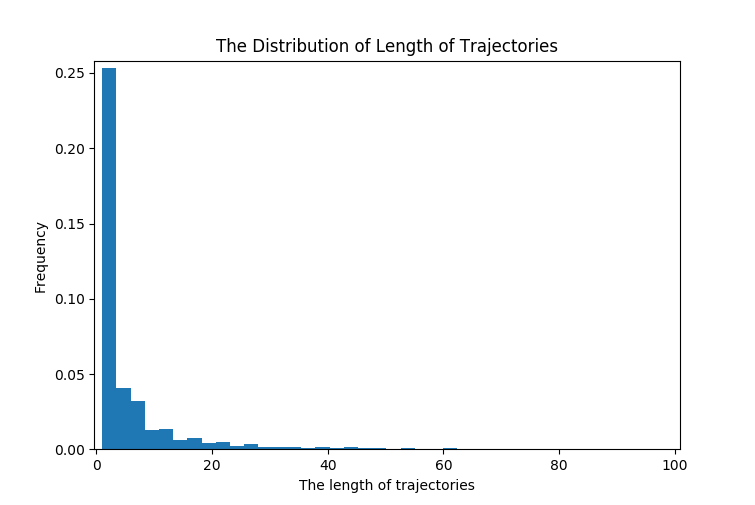
\includegraphics[scale=0.4]{hist.png}
    \caption{轨迹长度的分布情况(100以内)}
    \label{hist}
\end{figure}

为了得到较好的预测效果,后面会增加一些参数,尝试使用一些trick,并得到各参数对预测准确率的影响。

\section{基于Markov链的轨迹预测算法}
\subsection{问题描述}
轨迹预测的主要目的是:对未来用户的位置点进行预测。轨迹数据中的轨迹点对应于Markov链的状态。设已有用户的n个轨迹点,对应于k个位置,现在需要根据前n个轨迹点预测得到下一次用户会处于k个位置中的哪一个。

\subsection{基本思路}
基于Markov链的轨迹预测算法主要思路是:根据之前的轨迹点,统计得到转移概率矩阵P,并基于转移概率矩阵,对当前位置点的下一位置进行概率的计算,选择概率最大的位置点作为预测结果。

\subsection{问题描述}
设对于一个轨迹T,包含n个轨迹点,对应于k个地理位置,则转移概率矩阵是一个k$\times$k的矩阵,记为P。设矩阵P的第i行第j列为$p_{ij}$,表示位置i到位置j的概率,可以通过使用历史轨迹数据统计得到。

在已有的真实数据中,统计位置i转到位置j的次数,用$N_{ij}$表示,则:
\begin{equation}
	p_{ij} = \frac{N_{ij}}{\sum_{j=1}^{k}N_{ij}}  \quad 1\leq i, j\leq k
\end{equation}
由此就可以得到一步转移概率矩阵P。

虽然基于得到的一步转移概率矩阵已经可以对未来位置进行预测,但没有充分利用历史轨迹点带来的信息,因而可以保留h个历史轨迹点,使用\textbf{h步转移概率矩阵}进行预测,则:

\begin{equation}
	P(h)= P^{h}
\end{equation}

假设保留h步的历史轨迹,h步之前的轨迹点认为对未来位置的影响可以忽略不计。因而可以基于Markov链,使用加权的方式,时间越久远的数据权重越小,最后从概率向量中选择概率最大的位置作为预测结果,如果概率相同,则预测结果返回一个向量。

此处需要说明,在计算预测正确率时,只要\textbf{真实位置存在于预测向量中,则认为预测结果正确}。

\section{算法实现及结果}
\subsection{使用经纬度进行预测}
算法实现时使用的“tweets.txt”数据中,只有293559条数据含有准确的经纬度信息,其余数据可能在经纬度数据采集时出现了问题。因而,如何使用轨迹点的经纬度信息进行预测,只能\textbf{使用这29万多条数据}。

轨迹长度和经纬度的精度会对预测的效果产生较大的影响,尝试引入了两个参数,分别表示所使用的轨迹最短长度和经纬度的小数位数。表\ref{rlatlon}展示了不同参数下的用户平均预测准确率:第一列表示使用轨迹的最小长度,第一行表示经纬度的小数位数(给的数据小数位数为4)。

\begin{table}[!htbp]
  \centering  
  \begin{tabular}{c|c|c|c|c} 
  \hline
	    & 4 & 3 & 2 & 1 \\ \hline
	1	&	15.26\%	&	19.96\%	&	30.22\%	&	44.80\% \\
	10	&	23.34\%	&	29.24\%	&	38.65\%	&	59.73\% \\
	20	&	25.78\%	&	30.80\%	&	38.32\%	&	61.12\% \\
	50	&	28.28\%	&	30.74\%	&	38.32\%	&	63.61\% \\
  	\hline
  \end{tabular}
\caption{轨迹预测准确率:基于经纬度}
\label{rlatlon}
\end{table}

\subsection{使用POI进行预测}
“tweets.txt”数据中包含了POI信息,每个位置对应于唯一的POI。使用POI替代经纬度,使用基于Markov链的预测算法,得到表\ref{rPOI}所示的预测结果。

\begin{table}[!htbp]
  \centering  
  \begin{tabular}{c|c|c|c|c} 
	\hline
	最小轨迹长度	& 1	& 10 & 	20	& 50 \\ \hline
	准确率	& 14.4\% & 25.8\%	& 27.7\% & 27.0\% \\
	\hline
  \end{tabular}
\caption{轨迹预测准确率:基于POI}
\label{rPOI}
\end{table}
\end{document}}